\section{Results}

We used the Keras\footnote{\url{https://keras.io}} deep learning framework for implementing our neural networks. Keras is a high-level deep learning framework. It can use Theano\footnote{\url{http://deeplearning.net/software/theano/}} or TensorFlow\footnote{\url{https://www.tensorflow.org}} as its backend. We ran Keras on top of TensorFlow.

We used a server with a 64-bit Intel Xeon processor and 128GB RAM for training our networks. The training process took about 20 minutes for the sentiment analysis task and 60 minutes for the gender prediction task.

\subsection{Sentiment Analysis}

We trained our network for sentiment analysis with 200,000 reviews. We kept the labels balanced in our training set so that the number of reviews with positive ratings was the same as the number of reviews with negative ratings.

\subsubsection{Prediction Accuracy}

For our implementation, although our end goal was not to train a classifier that beat the best method for this dataset, we still wanted our model be as close to the best method as possible. The best accuracy so far for sentiment analysis on this data set has been 96\% \cite{Tang2015}. We were able to train a model whose validation accuracy is 93\%.

\subsubsection{Explanations Generated}

We generated explanations for the predictions made by our network for sentiment analysis using integrated gradients and 1-gram masking. Figure \ref{fig:sa:int-grad} shows examples of explanations generated by using integrated gradients. In particular, figure \ref{fig:sa:int-grad:pos} shows the explanations generated for a positive review and figure \ref{fig:sa:int-grad:neg} shows the explanations generated for a negative review. In figure \ref{fig:sa:int-grad:pos}, the words ``the'' and ``is'' have been assigned relatively lower weights while the words ``food'' and ``amazing'', which are words more central to the positive sentiment of this sentence, have been assigned higher weights. Similarly in figure \ref{fig:sa:int-grad:neg}, words such as ``really'', ``hate'' and ``tastes'' have been assigned higher weights than the other words because they 
have a higher influence in causing this review to be negative.

Figure \ref{fig:sa:mask} shows examples of explanations generated by using 1-gram masking. More specifically, figure \ref{fig:sa:mask:neg} shows the explanations generated for a negative review and figure \ref{fig:sa:mask:pos} shows the explanations generated for a positive review. The red horizontal line in these figures shows the prediction score for the complete review text without any of the words being masked. As words in the review text are masked, the prediction score changes. The prediction score obtained by masking a particular word is shown by the bar corresponding to that word. Words which cause a higher change in the prediction score are more central to determining the sentiment associated with the review text. Thus, the word ``disappointing'' has a higher relevance for explaining the negative sentiment in figure \ref{fig:sa:mask:neg}. Similarly, in figure \ref{fig:sa:mask:pos}, the word ``great'' (whose masking causes the greatest drop in the prediction score) is the most relevant for explaining the positive sentiment in the review. 

\begin{figure*}[t]
	\centering
	\begin{subfigure}{0.45\textwidth}
		\centering
		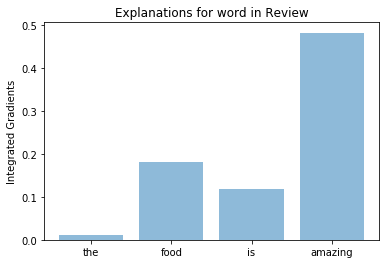
\includegraphics[width=\linewidth]{figure2}
		\caption{Positive review}
		\label{fig:sa:int-grad:pos}
	\end{subfigure} % There should be no newlines here.
	\begin{subfigure}{0.45\textwidth}
		\centering
		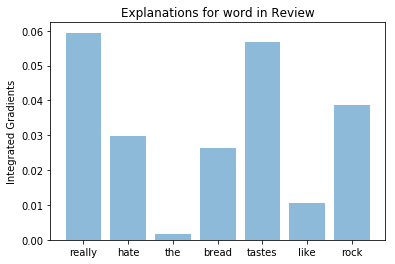
\includegraphics[width=\linewidth]{figure3}
		\caption{Negative review}
		\label{fig:sa:int-grad:neg}
	\end{subfigure}
	\caption{Explanations generated for sentiment analysis by using integrated gradients}
	\label{fig:sa:int-grad}
\end{figure*}

\begin{figure*}[t]
	\centering
	\begin{subfigure}{0.45\textwidth}
		\centering
		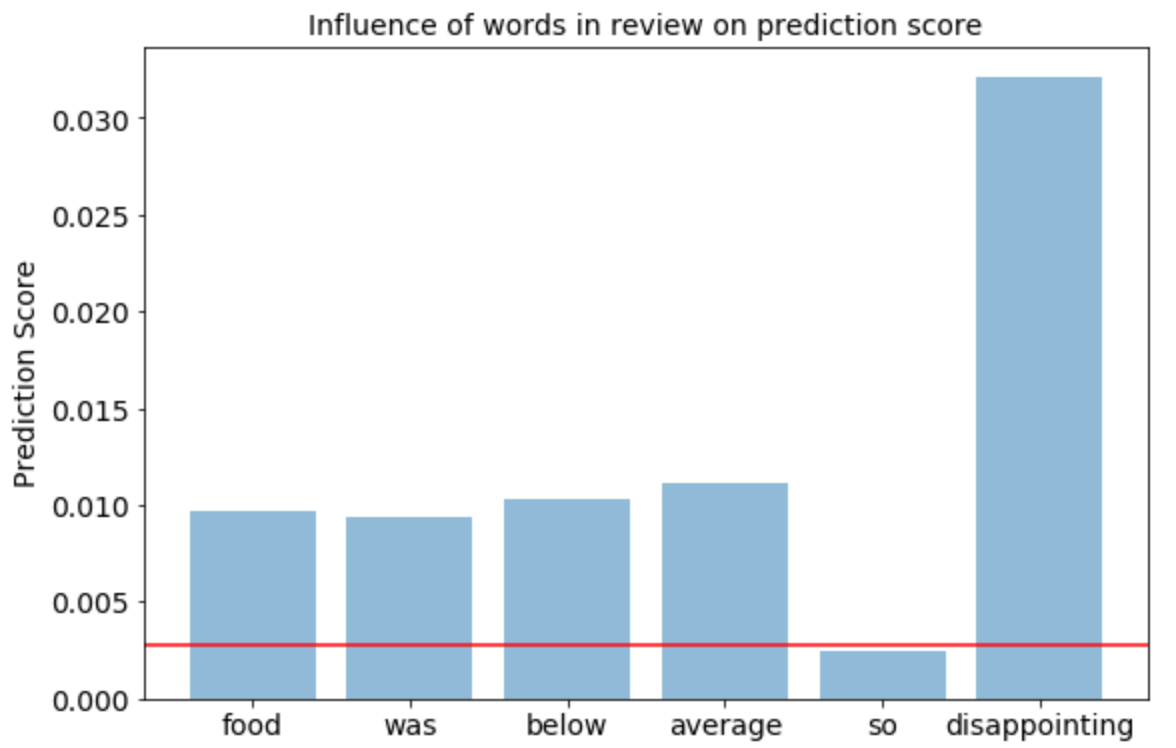
\includegraphics[width=\linewidth]{figure5}
		\caption{Negative review}
		\label{fig:sa:mask:neg}
	\end{subfigure} % There should be no newlines here.
	\begin{subfigure}{0.45\textwidth}
		\centering
		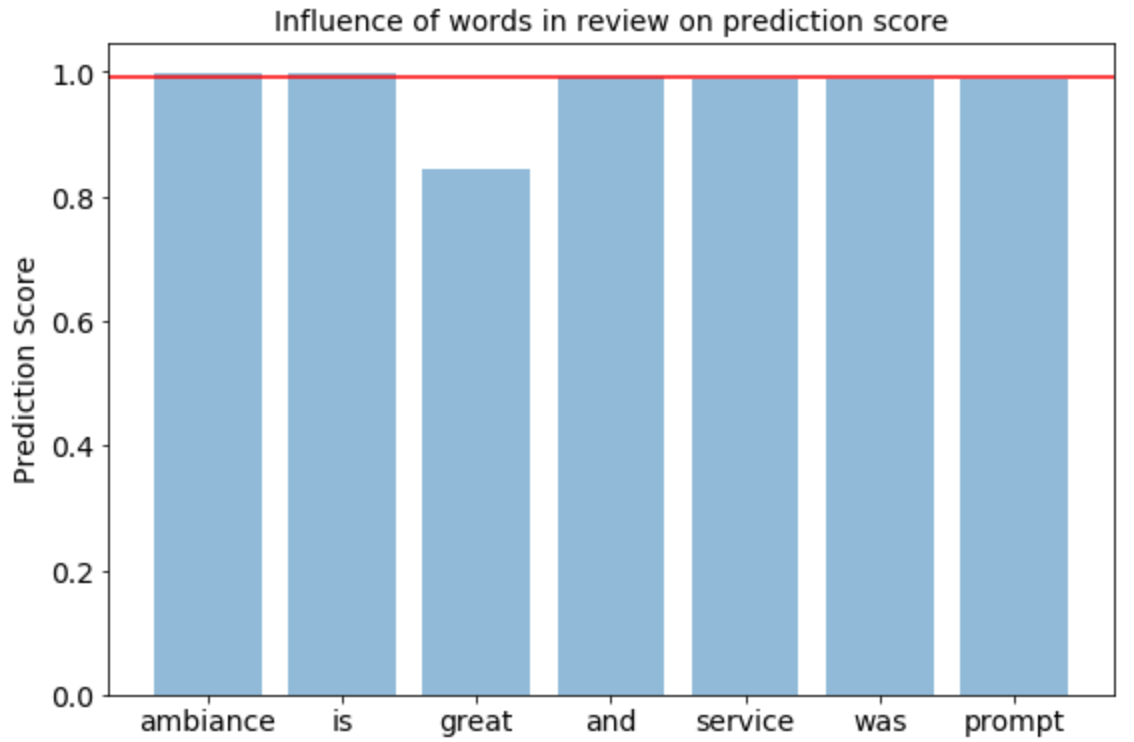
\includegraphics[width=\linewidth]{figure4}
		\caption{Positive review}
		\label{fig:sa:mask:pos}
	\end{subfigure}
	\caption{Explanations generated for sentiment analysis by using 1-gram masking}
	\label{fig:sa:mask}
\end{figure*}

\subsection{Gender Prediction}

 As mentioned in section \ref{subsection:gp}, we trained two networks for gender prediction - one with individual reviews and the other with reviews of particular users combined together. We used 500,000 reviews for training the network for gender prediction using single reviews. We trained the network for gender prediction on combined reviews using 50,000 instances. In both cases, we kept the labels in our training set balanced. In other words, the number of instances corresponding to male reviewers was the same as the number of instances corresponding to female reviewers.

\subsubsection{Prediction Accuracy}

We achieved a classification accuracy of 69.5\% for single reviews, and 84.5\% for combine reviews. This is comparable to the accuracy of state-of-the-art neural networks that have been used to predict the gender of authors of blog posts and tweets \cite{Burger2011, Mukherjee2010}.

\subsubsection{Explanations Generated}

As in sentiment analysis, we used integrated gradients and 1-gram masking to generate explanations for the gender prediction task as well. Figure \ref{fig:gp:int-grad} shows examples of explanations generated by using integrated gradients. The integrated gradients with respect to each word in a review text written by a female reviewer is shown in figure \ref{fig:gp:int-grad:female}. The word ``nail'' is the most prominent word in this review. Similarly, figure \ref{fig:gp:int-grad:male} shows the integrated gradients with respect to each word in a review given by a male reviewer. The word ``wife'' is the most influential for explaining the prediction for this review.

Figure \ref{fig:gp:mask} shows examples of explanations generated by using 1-gram masking. In particular, figure \ref{fig:gp:mask:female} shows the changes in the prediction score caused by masking each word in a review given by a female reviewer. In this case, the prediction of the original review text is greater than 0.5 (shown by the horizontal red line). The masking of the word ``nails'' causes the largest drop in the prediction score. So, it is the most influential word that causes this review to be classified as written by a female person. Similarly, figure \ref{fig:gp:mask:male} shows the changes in the prediction score brought about by the masking of each word in a review written by a male reviewer. The prediction score of the original review text, in this case, is less than 0.5. The largest increase in the prediction score is caused by the masking of the word ``girlfriend''. Therefore, it is the most influential word in determining the gender of the writer of this review.

It is interesting to note that in all of the above examples, the neural network used semantic content of the review (e.g. women visit nail salons, men have wives or girlfriends, etc.) to determine if a reviewer was male or female.

\begin{figure*}[t]
	\centering
	\begin{subfigure}{0.45\textwidth}
		\centering
		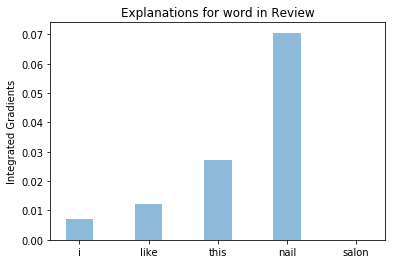
\includegraphics[width=\linewidth]{figure9}
		\caption{Female reviewer}
		\label{fig:gp:int-grad:female}
	\end{subfigure} % There should be no newlines here.
	\begin{subfigure}{0.45\textwidth}
		\centering
		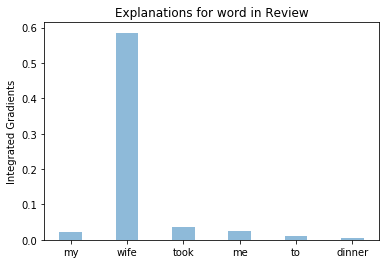
\includegraphics[width=\linewidth]{figure8}
		\caption{Male reviewer}
		\label{fig:gp:int-grad:male}
	\end{subfigure}
	\caption{Explanations generated for gender prediction by using 1-gram masking}
	\label{fig:gp:int-grad}
\end{figure*}

\begin{figure*}[t]
	\centering
	\begin{subfigure}{0.45\textwidth}
		\centering
		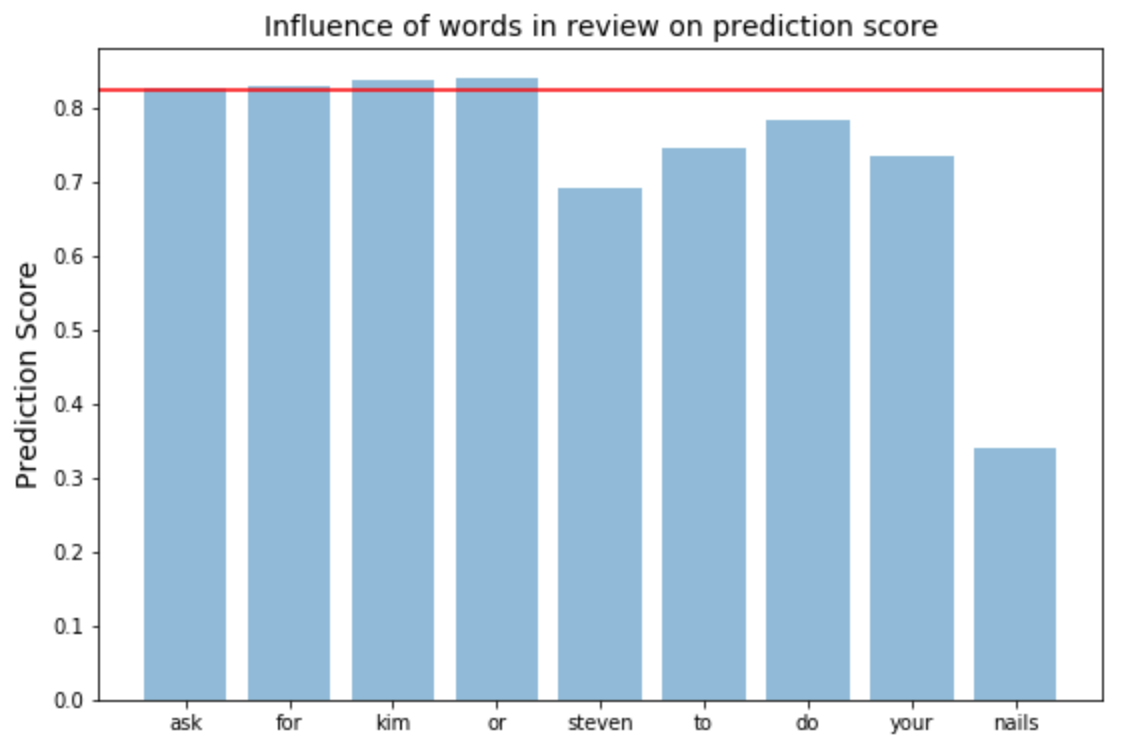
\includegraphics[width=\linewidth]{figure7}
		\caption{Female reviewer}
		\label{fig:gp:mask:female}
	\end{subfigure} % There should be no newlines here.
	\begin{subfigure}{0.45\textwidth}
		\centering
		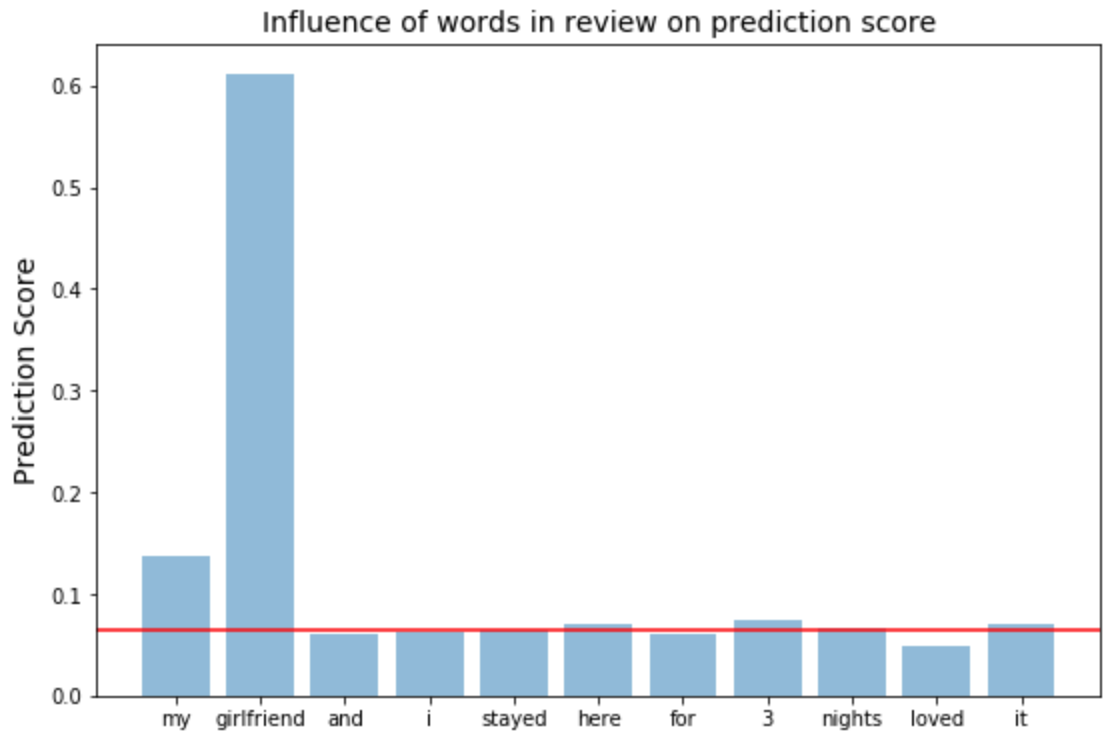
\includegraphics[width=\linewidth]{figure6}
		\caption{Male reviewer}
		\label{fig:gp:mask:male}
	\end{subfigure}
	\caption{Explanations generated for gender prediction by using 1-gram masking}
	\label{fig:gp:mask}
\end{figure*}

\subsubsection{Gender Bias}

We also tested the networks that we trained for gender prediction to see if they could detect stylistic differences between reviews from men and those written by women. We found some interesting examples of stylistic differences in the Yelp dataset. Table \ref{table:bias} shows an example in which the model exhibits gender bias by assigning higher probabilities to sentences with phrases like ``oh my god'' or ``sooooo'' causing the review to be classified as written by a female reviewer. The biases are likely learned by the system from similar instances in the training data that are written by female reviewers.

In figure \ref{fig:bias}, using the integrated gradients method, we can see that the word ``soooo'' is the most influential word in causing the sentence to be classified as written by a female person. This indicates that the model we have trained exhibits gender bias.

\begin{table*}
    \centering
    \begin{tabular}{|l|l|}
    \hline
    Review Text & Prediction Score  \\
    \hline
    'the food is good' & 0.49949434 (Male)  \\
    \hline
    'Oh my god the food is good' & 0.56273288 (Female)    \\
    \hline
    'Oh my god the food is sooooo good' & 0.75836354 (Female) \\
    \hline
    'Oh my god the food is sooooo good! I love this place!!' & 0.84929174 (Female)   \\
    \hline
    \end{tabular}
    \caption{Gender bias exhibited by the system}
    \label{table:bias}
\end{table*}

\begin{figure}
	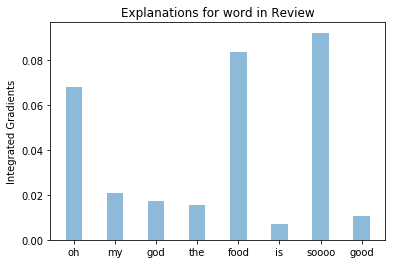
\includegraphics[width=\textwidth]{figure10}
	\caption{Explanation of Gender Bias}
	\label{fig:bias}
\end{figure}

\subsection{Effectiveness of Explanation Methods}

Despite the above results, the explanation models that we have used, namely integrated gradients and 1-gram masking, did not work well for all sentence instances that we tested. For example, integrated gradients does not work well when the review text is longer than a few words. The reason for this is that the points along the path from a baseline embedding vector to the actual embedding vector of a word are not in the distribution of an embedding at all. This is because all word embedding vectors are normalized to be on the radius-1 ball in the embedding space. So, if we normalize the points on the path, we essentially get the same vector; if we don't normalize it, we get vectors that are not in the distribution at all. As a result, integrated gradients used in an RNN language model may not perform as well as it does in image-related tasks.

The performance of 1-gram masking also varies greatly with the sentence or task. Often, there is a collection of words such that masking individual words does not change the prediction score much but masking them all introduces a significant change in the prediction score. Moreover, the order of words in a review text is also important. In addition, removing a word will necessarily break the distribution faithfulness since the sentence will likely become ungrammatical. Because of these reasons, simply removing a word will not necessarily create a good counter-factual for the sentence with regard to that word. 1-gram masking worked well in our examples because a single word had a large influence in making a prediction and masking it caused a drastic change in the prediction score. In gender prediction, for example, words such as ``husband'', ``wife'' and ``nails'' are semantically influential words in determining the reviewer's gender and exert a large influence on the prediction score. These words are stronger hints than stylistic word choices, thus accumulating most of the influence, thereby causing the explanation models to work really well.

In addition to integrated gradients and 1-gram masking, we also explored the use of \textit{Quantitative Input Analysis (QII)} \cite{Datta2017} for explaining machine learning models. QII uses a similar causal intervention mechanism as integrated gradients. It randomly intervenes on a single input or on multiple inputs by sampling from their distribution. It then inspects the influence of each input by looking at the outputs in relation to the casual intervention. However, it is hard to obtain a distribution for a single word in a sentence context. If we define the distribution based on the distance from the embedding vector, words that are close together can have a huge difference in the influence on the prediction for a sentence. For example, in the sentence \textit{The food is tasty}, if we intervene on the word \textit{tasty}, we can get both \textit{nasty} and \textit{delicious}, which are both close to the word \textit{tasty} in the embedding space. But we can expect these two interventions to have totally different outcomes. Thus, it is difficult to generate counterfactuals for words in a sentence, as the distribution of words in the embedding space is not always the ideal distribution for a certain task.
